\section{Design}
\label{sec:design}

In this section, we begin with describing PathSim framework in greated detail.
Then, we will delve into the changes that we made to the PathSim framework to
implement a more efficient similarity search framework while being able to
support hints and OLAP operations from the user.

\subsection{PathSim}

PathSim is developed to compute
similarity measures in a heterogeneous information network which are logical
networks that involve multiple typed vertices and multiple typed links denoting
different relations (e.g., bibliographic network, news articles).

Figure~\ref{fig:relationship} shows an example heterogeneous information
network.  In this figure, there are 4 possible types of entities, author,
paper, venue and term, which are inter-connected while there are also 4
different type of edges that exist (i.e., ''Writes``, ''Has``, ''Cited`` and
''Submitted To``).

\begin{figure}[H]
    \centering
    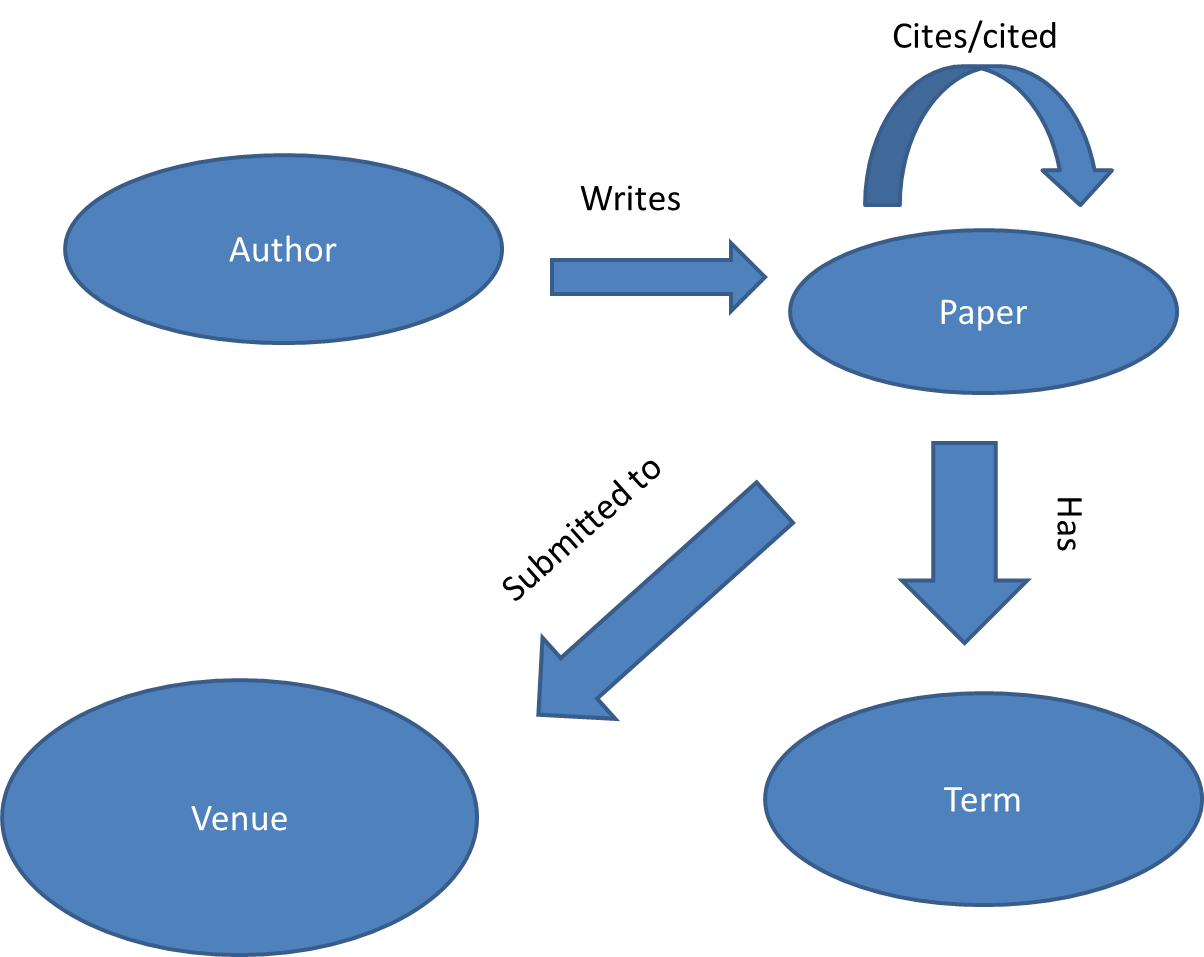
\includegraphics[width=0.6\linewidth]{./figs/relationship.png}
    \caption{Bibliographic Network}
    \label{fig:relationship}
\end{figure}

PathSim strives to define similarity measures between vertices in heterogeneous
information network using structural information and to answer top-k similarity
search queries efficiently. It accomplishes this by developing a novel meta
path-based framework.

As shown in Figure~\ref{fig:relationship}, entities can be connected via
different connectivity paths. For instance, two authors can be connected via
author-paper-author (i.e. co-authors) path or author-paper-venue-paper-author
(i.e.  the authors submitted both of their papers to the same conferences)
path. Intuitively, the different paths represent a different similarity
semantics. More formally, as written in the paper, the meta path can be
described as follows:

\begin{Def}
\label{meta path}
\textbf{Meta path}. A meta path $\mathcal{P}$ is a path defined on the graph on
network schema $\mathcal{T_G} = \mathcal{(A, R)}$, and is denoted in the form
of $\mathcal{A}_1 \xrightarrow{R_1} \mathcal{A}_2 \xrightarrow{R_2} \cdots
\xrightarrow{R_l} \mathcal{A}_{l + 1}$ which defines a composite relation
$\mathcal{R} = \mathcal{R}_1 \circ \mathcal{R}_2 \circ \cdots \circ
\mathcal{R}_l$ where $\circ$ denotes the composition operator on relations.
\end{Def}

Although multiple similarities measure have been previously explored such as
path counting or random walk-based similarity, they are biased to either
popular entities and thus unable to capture the essence of peer similarity.
For instance, if we would like to find out about authors that are similar to
an early PhD student that has published a few papers, the above measures
will yield professors who happen to co-author with this particular student
although what we desire are other PhD students. This has become the other
motivation for PathSim. Using the concept of meta path above, Path-Sim
defines the relationship between two entities as follow:

\begin{Def}
\label{path-sim}
PathSim: A meta path based similarity measure. Given a symmetric
meta path $\mathcal{P}$, PathSim between two vertices of the same type
x and y is:

\paragraph{}$s(x,y)=\frac{2*|\{p_{x \rightsquigarrow x}:p_{x \rightsquigarrow y}\}|\in\mathcal{P}}
{|\{p_{x \rightsquigarrow x}:p_{x \rightsquigarrow x}\}|\in\mathcal{P} +
|\{p_{y \rightsquigarrow y}:p_{y \rightsquigarrow y}\}|\in\mathcal{P}}$, where $p_{a \rightsquigarrow b}$ is the meta paths between $a$ and $b$.
\end{Def}

Intuitively, this indicates that if $x$ is popular, but not $y$, the number of
meta paths between $x$ and itself will be much larger than the number of
meta paths between $x$ and $y$. Thus, when we are comparing a popular entity
and an un-popular entity $s(x,y)$ will be low and vice versa. We need to have
either both to be popular or un-popular so that $s(x,y)$ yield a considerable
value.

\subsection{hPathSim}

There are three main improvements that we made to the PathSim framework.
Firstly, even with the pruning algorithm that they introduce in the paper,
the original PathSim framework still requires expensive matrix computations
that are not feasible in an online setting. We introduce a better storage
mechanism, \mTable, that allows faster materialization of the meta paths. Secondly,
we built our own tree data structure, \hTable, to allow us to perform
efficient OLAP operations on the dataset. Thirdly, we show how we are able
to support user defined constraints in our dataset.

% Depending on the meta path that it wants to materialize

\subsubsection{Storage Optimization}

In \h, we introduce a hash-table in which the key is a pair of node,
$(\mathcal{N}_1, \mathcal{N}_2)$ while the value is a set of meta paths between
the pair.  At first, the hash-table is empty. But as user queries for
similarity measures on two vertices in the graph, meta-paths found during the
computation will be cached in the hash-table. This enables fast retrieval if
the user issues the same queries in the future.

However, as noted in the original PathSim paper, it is impossible to cache all
of the possible meta-paths in an enormous graph. The author of the paper
calculated the storage size requirement of all the possible length-4 meta paths
in the DBLP data set is more than 40GB. Thus, we use an underlying database in
our framework to regularly swap meta paths in the cache to the disk if we are
using too much memory. We use Least Recently Used (LRU) policy to determine
which meta paths that need to be swapped to the disk due to its simplicity and
its effectiveness in ensuring that it works.

The database is checked every time the user issues a similarity search query to
see if meta paths between two vertices have been computed previously. If so, the
meta paths will be swapped back to the cache again. Similar to our cache, the
database will still be indexed by $(\mathcal{N}_1, \mathcal{N}_2)$ to allow
fast retrieval.

\subsubsection{Hierarchy Forest}
\label{sec:hier_forest}

The heterogeneous network contains hierarchies for certain entities. For example,
a location hierarchy could look like:

\begin{align*}
Urbana \leadsto USA \leadsto North America \leadsto root
\end{align*}

\h builds a forest of hierarchical trees, the trees are using HashTables in their core to
allow for fast lookup of a node in the tree. The roll-up and drill-down operations
on the tree are implemented just by using a depth-first search (DFS).

The forest provides 5 key operations for each of the trees:
\begin{itemize}
    \item \textit{is\_member(nodeTitle, queryID)}: Applies an iterative DFS to check if
    the node with id \textit{queryID} is under the subtree of \textit{nodeTitle}.
    \item \textit{is\_slice(nodeTitle, queryID)}: check whether the node with $nodeTitle$
    has the id $queryID$.
    \item \textit{get\_categories()}: return the tree titles in the forest.
    \item \textit{get\_children(nodeTitle)}: get all immediate children under the node
    $nodeTitle$.
    \item \textit{get\_parent(nodeTitle)}: get the parent of the node $nodeTitle$.
\end{itemize}

All the operations described above take $O(1)$ run-time due to the HashTable, except for
\textit{is\_member} which can take $O(N)$ where $N$ is the number of nodes under the specified
hierarchy tree.

\subsubsection{User-Specified Constraints}
\label{sec:user_constraint}

Thirdly, we also allow user to specify constraints on the type of meta paths
result that are used for computing the similarity score. There are two types of
constraints that the user could specify. Firstly, a user could specify that
meta paths between two vertices must go through a certain node or any nodes
with a particular category type. Conversely,  a user could also specify that
meta paths between two vertices must not go through a certain node or any nodes
with a particular category type. We choose these two types of constraints
becaues we believe that they are intuitive for the users and will allow users
to identify similarity between the two objects in a greater detail. These
constraints are stored in a hash-table, \cTable.

Similar to the original PathSim framework, the top-k paths used for the
similarity search computation are discovered through a Breadth-First Search
(BFS) algorithm. We based our algorithm off BFS due to its simplicity and guarantee to
compute shortest path between two vertices. The first constraint is being
enforced as we add a node into our candidate set

\begin{algorithm}
    \caption{Constrained BFS Algorithm to Find Meta-Paths}
    \label{alg:1}
    \begin{algorithmic}[1]
        \Function{FindPath}{c, src, dst}
            \State q $\gets$ Queue()
            \State paths $\gets$ Set()
            \State q.enqueue(Array(src))
            \State
            \While {not q.empty()}
                \State curPath $\gets$ q.dequeue()
                \State lastNode $\gets$ curPath.lastNode
                \For {n $\leftarrow$ lastNode.neighbors}
                    \If{check(n, c, "mustNotHave")}
                        \State continue
                    \ElsIf{n in curPath}
                        \State continue
                    \EndIf
                    \State

                    \State newPath $\gets$ curPath.append(n)

                    \If{n $==$ dst}
                        \If{check(n, c, "mustHave")}
                            \State paths.add(newPath)
                        \EndIf
                    \Else
                        \State q.enqueue(newPath)
                    \EndIf
                \EndFor
            \EndWhile
            \State
            \State \Return{paths}
        \EndFunction
    \end{algorithmic}
\end{algorithm}

Algorithm~\ref{alg:1} shows the algorithm that we use to discover the top-k
paths with user-specified constraints. The first $check$ function
is called every time a new partial path is explored. It ensures that nodes
that user \textit{does not want} to be added are being pruned from the search
space to save computation time. The second $check$ function
is called only when a full candidate path between the source and destination
is discovered. This ensures that all the nodes that the user \textit{wants}
exist in the path.
